\documentclass[twoside, letterpaper, 12pt]{report}
\usepackage{orthodoxservicebook}

\title{The Sunday Reader's Service of the \\ \textsc{Typica} \\ 2020 May 17}
\titlepic{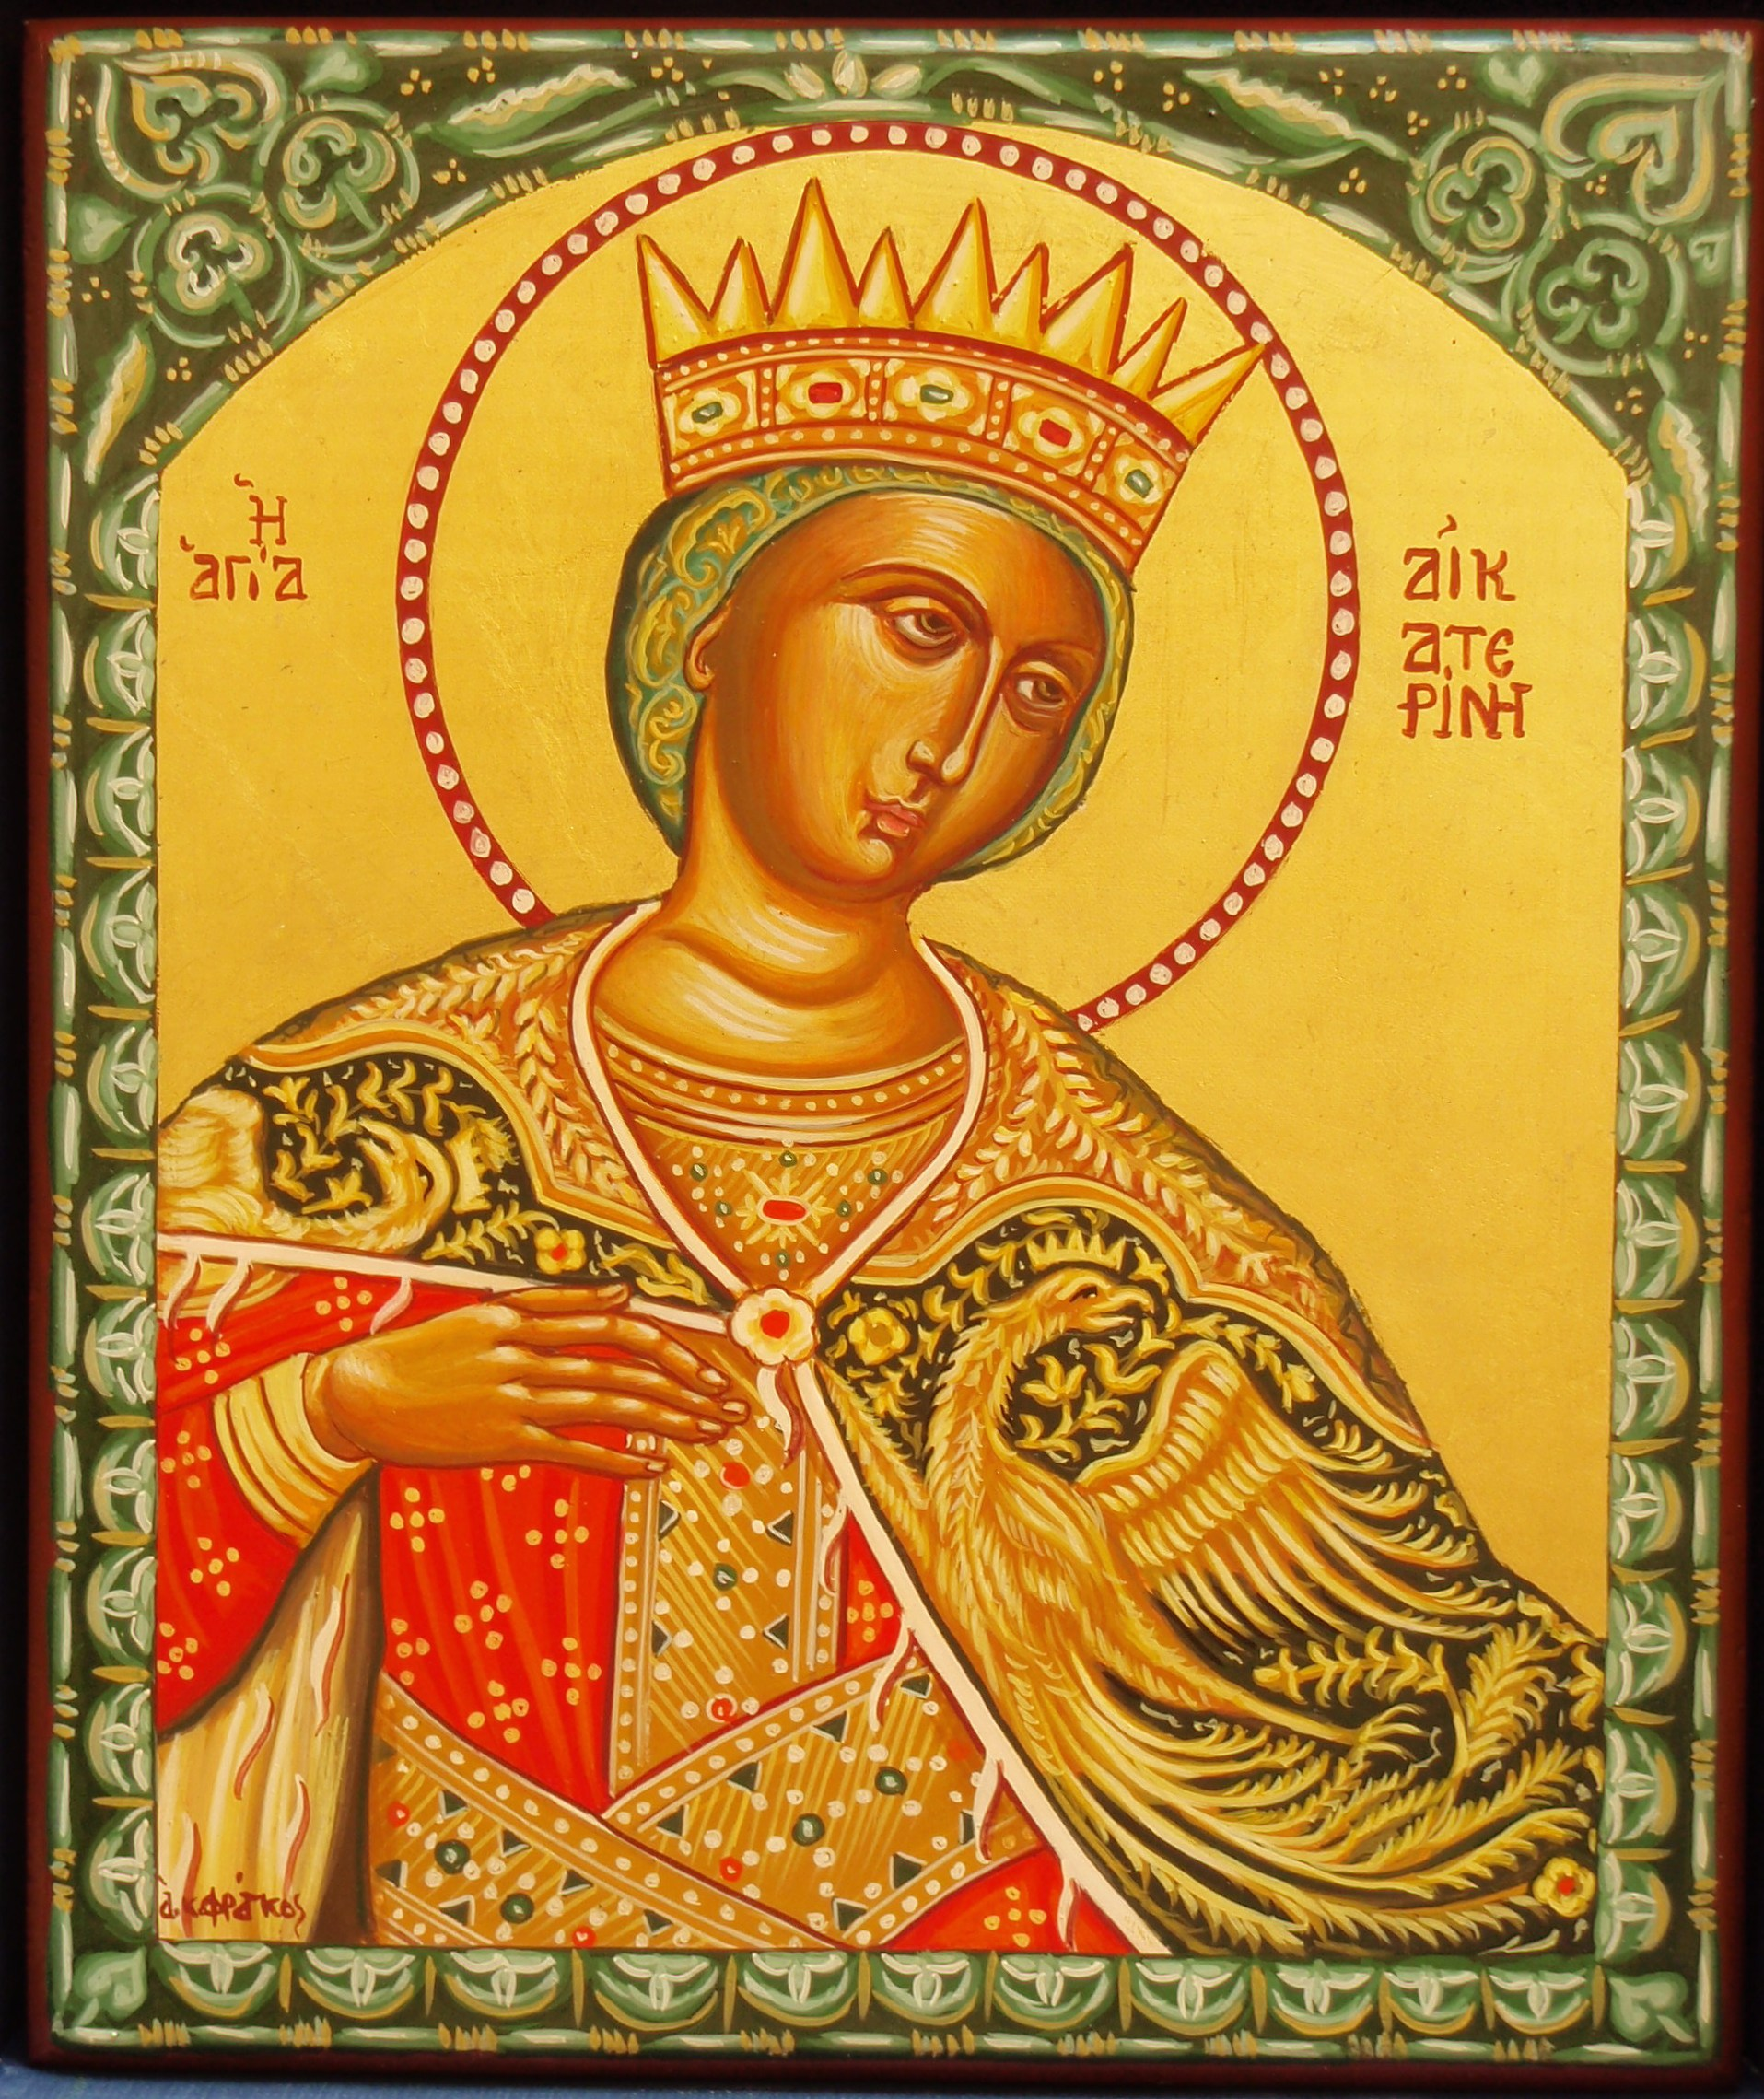
\includegraphics[width=0.5\textwidth]{Katherine1.jpg}}
\date{}
\author{}

\begin{document}
\maketitle
\pagestyle{empty} % Don't show page numbers
\instruction{This page intentionally left blank}
\cleardoublepage
\pagestyle{plain}
\setcounter{page}{1} % Set the page counter to 1 on the first real page
\chapter*{Service of Typica on Sunday, May 17}
\instruction{Fifth Sunday of Pascha - After-feast of Mid-Pentecost\\
Sunday of the Samaritan Woman}

\readerline{\throughtheprayers{}}
\choralresponse{./Z-Responses/Obikhod/Amen.ly}

\trisagionNeedsAmen[reader][prepentecost]

\choralresponse{./Z-Responses/Obikhod/Amen.ly}


\centeredsection{The First Antiphon}
\lilypondfile{./Liturgy/B-FirstAntiphon/BlessTheLord_Greek-Music.ly}

\centeredsection{The Second Antiphon}
\lilypondfile{./Liturgy/C-SecondAntiphon/PraiseTheLord_Greek-Music.ly}

\centeredsection{The Third Antiphon}
\lilypondfile{./Liturgy/D-ThirdAntiphon/Beatitudes_Moscow-Music.ly}

\centeredsection{The Epistle}

\instruction{Both of the New Testament lessons are read
without liturgical introduction or conclusion.
The readers start with “The Reading from…” and proceeds}

\paragraph{The Reading from the Acts of the Saintly and Pure Apostles. (11:19-30)}\mbox{}\\

\begin{maybetwocolumns}
  In those days, the Disciples, who were scattered because of the persecution that arose over
  Stephen, traveled as far as Phoenicia and Cyprus and Antioch, speaking the Word to none except
  Jews. But there were some of them, men of Cyprus and Cyrene, who, upon coming to Antioch,
  spoke to the Greeks also, preaching the Lord Jesus. And the hand of the Lord was with them, and
  a great number that believed turned to the Lord. News of this came to the ears of the church in
  Jerusalem, and they sent Barnabas to Antioch. When he came and saw the grace of God, he was
  glad; and he exhorted them all to remain faithful to the Lord with steadfast purpose; for he was a
  good man, full of the Holy Spirit and of faith. And a large company was added to the Lord. So
  Barnabas went to Tarsus to look for Saul; and when he had found him, he brought him to Antioch.
  For a whole year they met with the church, and taught a large company of people; and in Antioch
  the Disciples were for the first time called Christians. Now in these days prophets came down from
  Jerusalem to Antioch. And one of them named Agabus stood up and foretold by the Spirit that
  there would be a great famine over all the world; and this took place in the days of Claudius. And
  the Disciples determined, every one according to his ability, to send relief to the brethren who
  lived in Judea; and they did so, sending it to the elders by the hand of Barnabas and Saul.
\end{maybetwocolumns}

\centeredsection{The Gospel}

\instruction{Both of the New Testament lessons are read
without liturgical introduction or conclusion.
The readers start with “The Reading from…” and proceeds}

\paragraph{The Reading from the Holy Gospel according to St. John. (4:5-42)}\mbox{}\\

\begin{maybetwocolumns}
  At that time, Jesus came to a city of Samaria, called Sychar, near the field that Jacob gave
  to his son Joseph. Jacob’s well was there, and so Jesus, wearied as He was with his journey, sat
  down beside the well. It was about the sixth hour. There came a woman of Samaria to draw water.
  Jesus said to her, “Give Me a drink.” For His Disciples had gone away into the city to buy food.
  The Samaritan woman said to Him, “How is it that Thou, a Jew, ask a drink of me, a woman of
  Samaria?” For Jews have no dealings with Samaritans. Jesus answered her, “If you knew the gift
  of God, and Who it is that is saying to you, ‘Give Me a drink,’ you would have asked Him, and
  He would have given you living water.” The woman said to Him, “Sir, Thou hast nothing to draw
  with, and the well is deep; where do you get that living water? Art Thou greater than our father
  Jacob, who gave us the well, and drank from it himself, and his sons, and his cattle?” Jesus said
  to her, “Everyone who drinks of this water will thirst again, but whoever drinks of the water that I
  shall give him will never thirst forever; the water that I shall give him will become in him a spring
  of water welling up to eternal life.” The woman said to Him, “Sir, give me this water, that I may
  not thirst, nor come here to draw.” Jesus said to her, “Go, call your husband, and come here.” The
  woman answered Him, “I have no husband.” Jesus said to her, “You are right in saying, ‘I have
  no husband’; for you have had five husbands, and he whom you now have is not your husband;
  this you said truly.” The woman said to Him, “Sir, I perceive that Thou art a prophet. Our fathers
  worshiped on this mountain; and Thou sayest that in Jerusalem is the place where men ought to
  worship.” Jesus said to her, “Woman, believe Me, the hour is coming when neither on this
  mountain nor in Jerusalem will you worship the Father. You worship what you do not know; we
  worship what we know, for salvation is from the Jews. But the hour is coming, and now is, when
  the true worshipers will worship the Father in spirit and truth, for such the Father seeks to worship
  Him. God is spirit, and those who worship Him must worship in spirit and truth.” The woman
  said to Him, “I know that Messiah is coming [He Who is called Christ]; when He comes, He will
  tell us all things.” Jesus said to her, “I Who speak to you am He.” Just then His Disciples came.
  They marveled that He was talking with a woman, but none said, “What dost Thou wish?” or,
  “Why art Thou talking with her?” So the woman left her water jar, and went away into the city,
  and said to the people, “Come, see a man Who told me all that I ever did. Can this be the Christ?”
  They went out of the city and were coming to Him. Meanwhile the Disciples besought Him,
  saying, “Rabbi, eat.” But He said to them, “I have food to eat of which you do not know.” So the
  Disciples said to one another, “Has anyone brought Him food?” Jesus said to them, “My food is
  to do the will of Him Who sent Me, and to accomplish His work. Do you not say, ‘There are yet
  four months, then comes the harvest’? I tell you, lift up your eyes, and see how the fields are
  already white for harvest. He who reaps receives wages, and gathers fruit for eternal life, so that
  sower and reaper may rejoice together. For here the saying holds true, ‘One sows and another
  reaps.’ I sent you to reap that for which you did not labor; others have labored, and you have
  entered into their labor.” Many Samaritans from that city believed in Him because of the woman’s
  testimony, “He said to me all that I ever did.” So when the Samaritans came to Him, they asked
  Him to stay with them; and He stayed there two days. And many more believed because of His
  words. They said to the woman, “It is no longer because of your words that we believe, for we
  have heard for ourselves, and we know that this is indeed the Savior of the world.”
\end{maybetwocolumns}

\centeredsection{Troparia Before the Creed}
\instruction{Plain reading}
\begin{reader}
\item[Reader 1:] The heavenly choir singeth thy praises, saying:
  Holy, holy, holy, Lord of Sabaoth; heaven and earth are full of Thy glory.

\item[Reader 2:] \emph{Come unto him, and be enlightened,
               and your faces shall not be ashamed.}
  The heavenly choir singeth thy praises, saying:
  Holy, holy, holy, Lord of Sabaoth; heaven and earth are full of Thy glory.

\item[Reader 1:] \emph{\glory}
  The choir of the holy angels and archangels,
  with all the powers of heaven, singeth thy praises, saying:
  Holy, holy, holy, Lord of Sabaoth; heaven and earth are full of Thy glory.

\item[Reader 2:]\emph{\nowandever}
\end{reader}

\centeredsection{The Creed}
\input{Common/TheCreed.txt}


\centeredsection{Prayer of Forgiveness}
\readerline{Forgive, remit, pardon, O God, our sins,
  both voluntary and involuntary, in deed and in word, in knowledge or in ignorance,
  committed by night or by day, in mind and in thought.
  Forgive us them all, for thou art good and lovest mankind.
}


\centeredsection{The Lord’s Prayer}
\input{Common/LordsPrayer.txt}

\readerline{Through the prayers of our holy fathers, Lord Jesus Christ our God, have mercy on us.}
\choralresponse{./Z-Responses/Obikhod/Amen.ly}


\centeredsection{Kontakia for Pascha in Tone 8}
\lilypondfile{./Pentecostarion/Pascha/Pascha-Kontakion-T8-Byz-Karam-Music.ly}

\readerline{\lhmForty}

\readerline{
  O Christ our God, Who art worshipped and glorified at all times at every hour both in
  heaven and on earth; Who art long-suffering and plenteous in mercy and compassion; Who lovest
  the just man and showest mercy upon the sinner; and Who callest all men to repentance through 
  the promise of blessings to come; receive, O Lord, at this very hour our supplications, and direct
  our lives in the way of Thy commandments: sanctify our souls, purify our bodies, set our minds
  aright, cleanse our thoughts; deliver us from all affliction, trouble, and distress; compass us about
  with Thy holy angels, that, guided and guarded by them, we may attain unto the unity of the Faith,
  and to the knowledge of Thine unapproachable glory; for Thou art blessed unto ages of ages. Amen.
}

\begin{reader}
  \item \lhmThree{}\\\emph{\gne{}}
  \item \morehonorablethanthetherubim{}
  \item \throughtheprayers{}
\end{reader}

\begin{maybetwocolumns}
\choralresponse{./Z-Responses/Obikhod/Amen.ly}

\readerline{\blessedbethename{}\thrice{}}

\centeredsection{Psalm 33}
\input{./Psalms/Psalm033-unknowntrans.txt}

\end{maybetwocolumns}

\peopleline{\gne}


\centeredsection{A Homily}
\begin{maybetwocolumns}
\instruction{The Courage to Face the Truth:\\
Homily for the Sunday of the Samaritan Woman in the Orthodox Church\\
Fr. Philip LeMasters, pastor, St. Luke Antiochian Orthodox Church of Abilene, Texas}

Christ is Risen! It is strangely appealing to define ourselves by our failures, especially
when others know that we have stumbled and treat us poorly as a result. As well, our own pride
often causes us to lose perspective such that we obsess about how we do not measure up to
whatever illusion of perfection we have accepted. People are often their own harshest critics in
ways that are not healthy at all.

On this Sunday of the Samaritan Woman, we celebrate that our Lord’s great victory over death
enables us to be free from defining ourselves by our sins or by how other people may view us. He
rises in glory not only over the tomb and Hades, but over all the distortions of the beauty of the
human person created in His image and likeness. Today we commemorate that His salvation
extends to our most painful failings and to the harsh judgments of others upon us. Even such
difficult circumstances may become points of entry into the joy of the empty tomb.

The woman at the well certainly knew what it was like to be defined by others as someone who
did not measure up. She was a Samaritan, and therefore rejected by the Jews as a heretic and a
member of a despised group that had intermarried with Gentiles. She herself had been married
five times and was now with a man to whom she was not married, which may have been why she
went to draw water at the unlikely time of high noon. Perhaps she went to the well in the heat of
the day in order to avoid the other Samaritan women who wanted nothing to do with someone like
her.

Imagine her surprise, then, when the Savior asked her for a drink of water and then engaged in a
conversation about spiritual matters with her. Jewish men simply did not strike up conversations
with women in that time and place, and consuming food or drink from a Samaritan was out of the
question. How even more shocking it is that Jesus Christ’s conversation with her is the longest
recorded between Him and any one person in the four gospels. He spoke straightforwardly to her
and did not shy away from uncomfortable truths that hit her where she lived. But instead of
shutting down the conversation or running away in fear, this Samaritan woman told the people of
her village about Christ. As a result, many of her neighbors came to believe in the Lord.

This Samaritan woman is known in the Church as St. Photini, which means “the enlightened one.”
Through the Savior’s conversation with her, Photini became an evangelist who boldly shared the
good news, even to her Samaritan neighbors who were surely used to viewing her in anything but
spiritual terms. That took tremendous courage. Photini was not only brave in preaching to them,
but ultimately in responding to the persecution of the pagan Roman emperor Nero, to whom she
said “O most impious of the blind, you profligate and stupid man! Do you think me so deluded
that I would consent to renounce my Lord Christ and instead offer sacrifice to idols as blind as
you?” The Great Martyr Photini refused to back down and gave the ultimate witness to Christ’s
victory over death by laying down her life for Him. The Savior had set her free even from fear of
the grave.

Too many of us today flee in shame from uncomfortable truths, whether we encounter them in our
own thoughts or in the opinions of others. Too many of us define ourselves by our failings,
weaknesses, and temptations. Too many of us accept some unrealistic cultural standard of “the
good life” as the norm we must meet in order to be worthwhile. Thank God, St. Photini the Great
Martyr did none of that. In response to her shocking encounter with the Savior, she humbly
acknowledged the truth about her brokenness; she did not react defensively or make excuses. She
did not end the conversation or run away in shame. Instead, she was open to the healing of her
soul, to the possibility of a new and restored life through the mercy of the Lord. This was such a
great blessing to her that she immediately shared the good news with the people of her village and
refused to stop, even to the point of laying down her life.

In this joyous season of Pascha, we celebrate that Christ’s victory over death delivers us from all
the corrupting effects of sin, including our deeply ingrained habits of thought and action that
distract us from facing the truth about ourselves. By setting us free from bondage to the fear of
death, our Risen Lord enables us to make even our most bitter failures points of entry into the new
day of His eternal life. He has conquered death, the wages of sin, which means that our sins now
have only the power over us that we allow them to have. When, like St. Photini, we acknowledge
them straightforwardly and turn away from them, we participate personally in the good news of
Pascha. We rise from death to life as we enter into the joy of the empty tomb. But when we
proudly refuse to confess or repent of our sins, we remain in slavery to our self-centered illusions
of perfection, to our sense of shame that we do not live up to the standards that we think we must
meet in order to be worthwhile.

In other words, we insist on being our own saviors. But since we cannot conquer death or heal our
own souls, that is nothing but foolish pride that keeps us bound to the fear of death, to the terror
of realizing how weak we are before the challenges we encounter both within our own minds and
in relation to others. Our failures and weaknesses are not good in and of themselves, but we put
them to good use when we let them open our eyes to the truth of who we are, of where we stand
before the Lord. If we will use them as ways to humble ourselves without making excuses or
otherwise blinding ourselves to what they reveal about us, then we will put ourselves in the blessed
place of St. Photini, who was thirsty for strength and healing that she knew she could not give
herself, for “a spring of water welling up to eternal life” from the depths of her soul.

Like her, we must refuse to be paralyzed by guilt and shame before others and in our own minds.
Then we will take our attention off whether we measure up to some self-imposed standard and
instead focus on receiving the healing mercy of Jesus Christ. No matter what we have done, no
matter how distorted and corrupt any dimension of our life may be, no matter how anyone else
treats or views us, Christ is able to raise us up with Him from death to life. That is not only a
future promise, but a present reality. He rose in glory with His wounds still visible, and no wound
that we or others have inflicted puts us beyond the good news of His resurrection. In this glorious
season of Pascha, let us all become like the Great Martyr Photini by embracing enthusiastically
the new life that the Savior has brought to the world, for Christ is Risen!
\end{maybetwocolumns}

\centeredsection{Ressurrectional Apolytikion in Tone 4}
\lilypondfile{./Octoechos/ResurrectionalApolytikion-Tone4-Kazan-Music.ly}

\centeredsection{Apolytikion for Mid-Pentecost in Tone 8}
In the midst of this Feast, O Savior, give Thou my thirsty soul to drink of the waters of true
worship; for Thou didst call out to all, saying: Whosoever is thirsty, let him come to Me and drink.
Wherefore, O Christ our God, Fountain of life, glory to Thee.

\centeredsection{Megalynarion of Sunday of the Samaritan Woman in Tone 1}
The angel spake to her that is full of grace, saying, O pure Virgin, rejoice; and I say also, Rejoice;
for thy Son is risen from the tomb on the third day.
Rejoice and be glad, O gate of the divine Light; for Jesus Who disappeared in the tomb hath risen
with greater radiance than the sun, illuminating all believers, O Lady favored of God.

\readerline{\throughtheprayers}

\choralresponse{./Z-Responses/Obikhod/Amen.ly}

\end{document}

